%!Mode::"UTF-8"
\documentclass[12pt]{article}

% 页面设置
\usepackage{geometry}
\geometry{left=2.5cm, right=2.5cm, top=2.5cm, bottom=2.5cm}
\usepackage{graphicx}
\usepackage{ctex}
\usepackage{fontspec}
\usepackage{setspace}

%高亮使用的颜色
\usepackage{xcolor}  	
\definecolor{commentcolor}{RGB}{0,121,121}
\definecolor{stringcolor}{RGB}{190,49,49}
\definecolor{keywordcolor}{RGB}{0,128,0}

% 代码设置
\usepackage{listings}
\usepackage{color}
\setmonofont{Consolas}
\definecolor{listing}{gray}{0.97}
\lstset{
	backgroundcolor=\color{listing},
	basicstyle=\footnotesize,
	commentstyle=\color{commentcolor},	%注释颜色
	keywordstyle=\color{keywordcolor}\textbf,	%关键词颜色
	stringstyle=\color{stringcolor},
	numbers=left,
	numberstyle=\footnotesize,
	stepnumber=1,
	aboveskip={0.5\baselineskip},
	belowskip={0.5\baselineskip},
	columns=fullflexible,
	breaklines=true,
	breakatwhitespace=true,
	frame=single,
	basicstyle=\ttfamily,
	numberstyle=\ttfamily,
	tabsize=3
}

% 字体设置
\setmainfont{Times New Roman}
\setCJKmainfont{SimSun}
\setCJKsansfont{SimHei}
\usepackage[version=4]{mhchem}
\usepackage{mathtools}
\usepackage{diffcoeff}

% 表格设置
\usepackage{makecell}
\newcommand{\addcell}[2][4]{\makecell{\zihao{#1}\textsf{#2}}}
\usepackage{titlesec}
\usepackage{booktabs}
\usepackage{tabularx}

% 设置图注、表注
\usepackage{caption}
\usepackage{bicaption}
\captionsetup{labelsep=quad, font={small, bf}, skip=2pt}
\DeclareCaptionOption{english}[]{
    \renewcommand\figurename{Fig.}
    \renewcommand\tablename{Table}
}
\captionsetup[bi-second]{english}

% 设置页眉
\usepackage{fancyhdr}
\pagestyle{fancy}
\fancypagestyle{preContent}{
    \fancyhead[L]{\zihao{-5} 机器学习基础}
    \fancyhead[C]{\zihao{-5} 作业5\ \ 支持向量机}
    \fancyhead[R]{\zihao{-5} 1800011828\ 王宇哲}
}
\pagestyle{preContent}

%	设置首页页眉页脚
\fancypagestyle{plain}{
	\fancyhead[L]{\zihao{-5} 机器学习基础}
	\fancyhead[C]{\zihao{-5} 作业5\ \ 支持向量机}
	\fancyhead[R]{\zihao{-5} 1800011828\ 王宇哲}
	\cfoot{}
}

% 设置标题格式
\titleformat*{\section}{\zihao{4}\sffamily}
\titleformat*{\subsection}{\zihao{-4}\sffamily}
\titleformat*{\subsubsection}{\zihao{-4}\sffamily}
\titlespacing*{\section}{0pt}{10pt}{10pt}
\titlespacing*{\subsection}{0pt}{10pt}{5pt}
\titlespacing*{\subsubsection}{0pt}{10pt}{5pt}

% 设置引用格式
\usepackage[super,round,comma,compress]{natbib}

\usepackage{amsmath}
\usepackage{amssymb}

%设置封面
\begin{document}
    % 标题页
    \begin{titlepage}
    	% 页眉
    	\thispagestyle{plain}
        % 图片
        \begin{figure}[h]
            \centering
            \includegraphics[width=0.7\textwidth]{pku.png}
        \end{figure}
        \vspace{60pt}
        % 标题
        \centerline{\zihao{-0} \textsf{机器学习基础}}
        \vspace{20pt} % 空行
        \centerline{\zihao{-0} \textsf{课程上机试验报告}}
        \vspace{70pt} % 空行
        \begin{center}
            \begin{tabular}{cp{5.5 cm}}
                % 题目
                \addcell[2]{{\Huge 试验内容:\ }} & \addcell[2]{{\Huge 支持向量机}} \\
                \cline{2-2}
            \end{tabular}
        \end{center}
        \vspace{60pt} % 空行
        \begin{center}
            \doublespacing
            \begin{tabular}{cp{5cm}}
                % 姓名
                \addcell{姓\phantom{空格}名:\ } & \addcell{王宇哲} \\
                \cline{2-2}
                % 学号
                \addcell{学\phantom{空格}号:\ } & \addcell{1800011828}\\
                \cline{2-2}
            \end{tabular}
        \end{center}
       
    \end{titlepage}

\section{题目6.2}
	\subsection{实验题目}
	试使用LIBSVM,在西瓜数据集$3.0\alpha$上分别用线性核和高斯核训练一个SVM,并比较其支持向量的差别。\par 西瓜数据集$3.0\alpha$见《机器学习》p.89的表4.5。

               
\vbox{}        
\subsection{实验数据}
题目6.2使用的数据集为周志华《机器学习》p.89所提供的西瓜数据集$3.0\alpha$,具体内容如\textbf{表1}所示。
\begin{table}[h]
	\centering
	\zihao{5}
	\bicaption{西瓜数据集$3.0\alpha$}{Watermelon dataset $3.0\alpha$}
	\begin{tabular}{ccccccccc}
		\toprule
		编号 & 密度 & 含糖率 & 好瓜 & & 编号 & 密度 & 含糖率 & 好瓜\\
		\midrule
		1 & 0.697 & 0.460 & 是 & & 9  & 0.666 & 0.091 & 否\\
		2 & 0.774 & 0.376 & 是 & & 10 & 0.243 & 0.267 & 否\\
		3 & 0.634 & 0.264 & 是 & & 11 & 0.245 & 0.057 & 否\\
		4 & 0.608 & 0.318 & 是 & & 12 & 0.343 & 0.099 & 否\\
		5 & 0.556 & 0.215 & 是 & & 13 & 0.639 & 0.161 & 否\\
		6 & 0.403 & 0.237 & 是 & & 14 & 0.657 & 0.198 & 否\\
		7 & 0.481 & 0.149 & 是 & & 15 & 0.360 & 0.370 & 否\\
		8 & 0.437 & 0.211 & 是 & & 16 & 0.593 & 0.042 & 否\\
		  &       &       &    & & 17 & 0.719 & 0.103 & 否\\
		\bottomrule
	\end{tabular}
\end{table}
\par

\vbox{}
\subsection{实验工具}
实验在个人LEVENO YOGA 710笔记本电脑上进行,主要硬件条件为:处理器Intel i5-7200U CPU,内存大小8.0 GB,显卡NVIDIA Geforce 940MX;操作系统为Windows 10 64位系统。\par 
实验使用语言为python,具体版本为python 3.7.0,通过Anaconda安装了Matplotlib、NumPy、pandas、scikit-learn等常用库。实验代码编写和运行均在Jupyter Notebook上进行,具体版本为Jupyter Notebook 6.3.0。

\vbox{}

\subsection{实验方法}
实验采用的算法为经典的支持向量机(SVM)算法。具体地,分别使用线性核(linear kernel)和高斯核(gaussian kernel)进行训练,引入超参数$C$作为正则化参数,以权衡对特异点的总的松弛程度和软间隔,得到软间隔支持向量机。经典SVM算法的原理在课程中已经进行详细讨论,此处不再赘述。\par
考虑到python sklearn库已集成了libsvm库,实验使用在libsvm基础上扩展形成的sklearn.svm库进行支持向量机的训练。sklearn.svm库支持使用核方法训练非线性支持向量机,可选的核包括线性核(linear kernel)、多项式核(polynomial kernel)、径向基函数核(rbf kernel)等。sklearn.svm库使用参数$C$进行正则化设置,$C$较大时对特异点的松弛幅度惩罚较大,默认$C=1.0$。\par 
实验的具体操作方法如下。首先将\textbf{表1}数据写入watermelon\_dataset.txt,导入实验所需的必要的库,并读取西瓜数据集$3.0\alpha$的数据:
\begin{lstlisting}[language=python]
	from matplotlib import pyplot as plt
	import pandas as pd
	import numpy as np

	with open('watermelon_dataset.txt', 'r') as dataset:
		X=[]
		y=[]
		while True:
			lines = dataset.readline()
			if not lines:
				break
				pass
			ID, density, sugar_content, label = [float(i) for i in lines.split()]
			X.append([density, sugar_content])
			y.append(int(label))
			pass
		X = np.array(X)
		y = np.array(y)
		pass
\end{lstlisting}
得到的X为西瓜数据集各样本的密度、含糖率组成的2维向量的集合,y为相应的各样本的类别标记的集合,“是好瓜”标记为+1,“不是好瓜”标记为-1。\par 
下面使用sklearn.svm库进行支持向量机的训练,并使用matplotlib库绘制出训练结果。一般地,首先定义函数svm\_train:
\\
\begin{lstlisting}[language=python]
	from sklearn import svm
	
	def svm_train(kernel='linear', C=1, label='label'):
	svc = svm.SVC(C=C, kernel=kernel, gamma=10)
	svc.fit(X, y)
	sv = svc.support_vectors_
	
	plt.figure()
	plt.clf()
	plt.scatter(X[:, 0], X[:, 1], c=y, zorder=10, cmap=plt.cm.Paired, edgecolor='k', s=30)
	plt.scatter(sv[:, 0], sv[:, 1], s=70, facecolors='none', zorder=10, edgecolor='k')
	
	plt.axis('tight')
	x_min = X[:, 0].min()
	x_max = X[:, 0].max()
	y_min = X[:, 1].min()
	y_max = X[:, 1].max()
	
	XX, YY = np.mgrid[x_min-0.2:x_max+0.2:200j, y_min-0.4:y_max+0.4:200j]
	Z = svc.decision_function(np.c_[XX.ravel(), YY.ravel()])
	
	Z = Z.reshape(XX.shape)
	plt.pcolormesh(XX, YY, Z > 0, cmap=plt.cm.Paired)
	plt.contour(XX, YY, Z, colors=['k', 'k', 'k'], linestyles=['--', '-', '--'], levels=[-.5, 0, .5])
	
	plt.title(label)
\end{lstlisting}
通过svm\_train函数实现支持向量机的训练和训练结果图的绘制,函数变量kernel指定所用的核,$C$为正则化参数,label为绘制的训练结果图的图题。训练结果图中标注了支持向量(双线空心圈)、未作为支持向量的训练样本(单线空心圈)、训练得到的分离超平面(黑色实线)和间隔边界(黑色虚线),并用不同颜色标注出正例点和负例点。\par 
最后分别用线性核和高斯核训练支持向量机,作出并保存训练结果图:
\begin{lstlisting}[language=python]
	svm_train(kernel='linear', C=1000, label='linear')
	plt.savefig('linear_result.jpg',dpi=1000, bbox_inches='tight')
	svm_train(kernel='rbf', C=1000, label='gaussian')
	plt.savefig('gaussian_result.jpg',dpi=1000, bbox_inches='tight')
	
	plt.show()
\end{lstlisting}
正则化参数$C=1000$通过实验过程中的多次尝试进行选取。在尝试增大$C$的过程中,$C=1000$时两支持向量机的训练结果与使用的支持向量个数均基本达到稳定,因此可以认为是较合理的正则化参数,此时两SVM均基本达到最优训练效果。
\vbox{}

\subsection{实验结果}
实验代码总运行时长为$2.17\ \ {\rm s}$。使用线性核训练得到的支持向量机的训练结果如\textbf{图1}所示。
\begin{figure}[h]
	\centering
	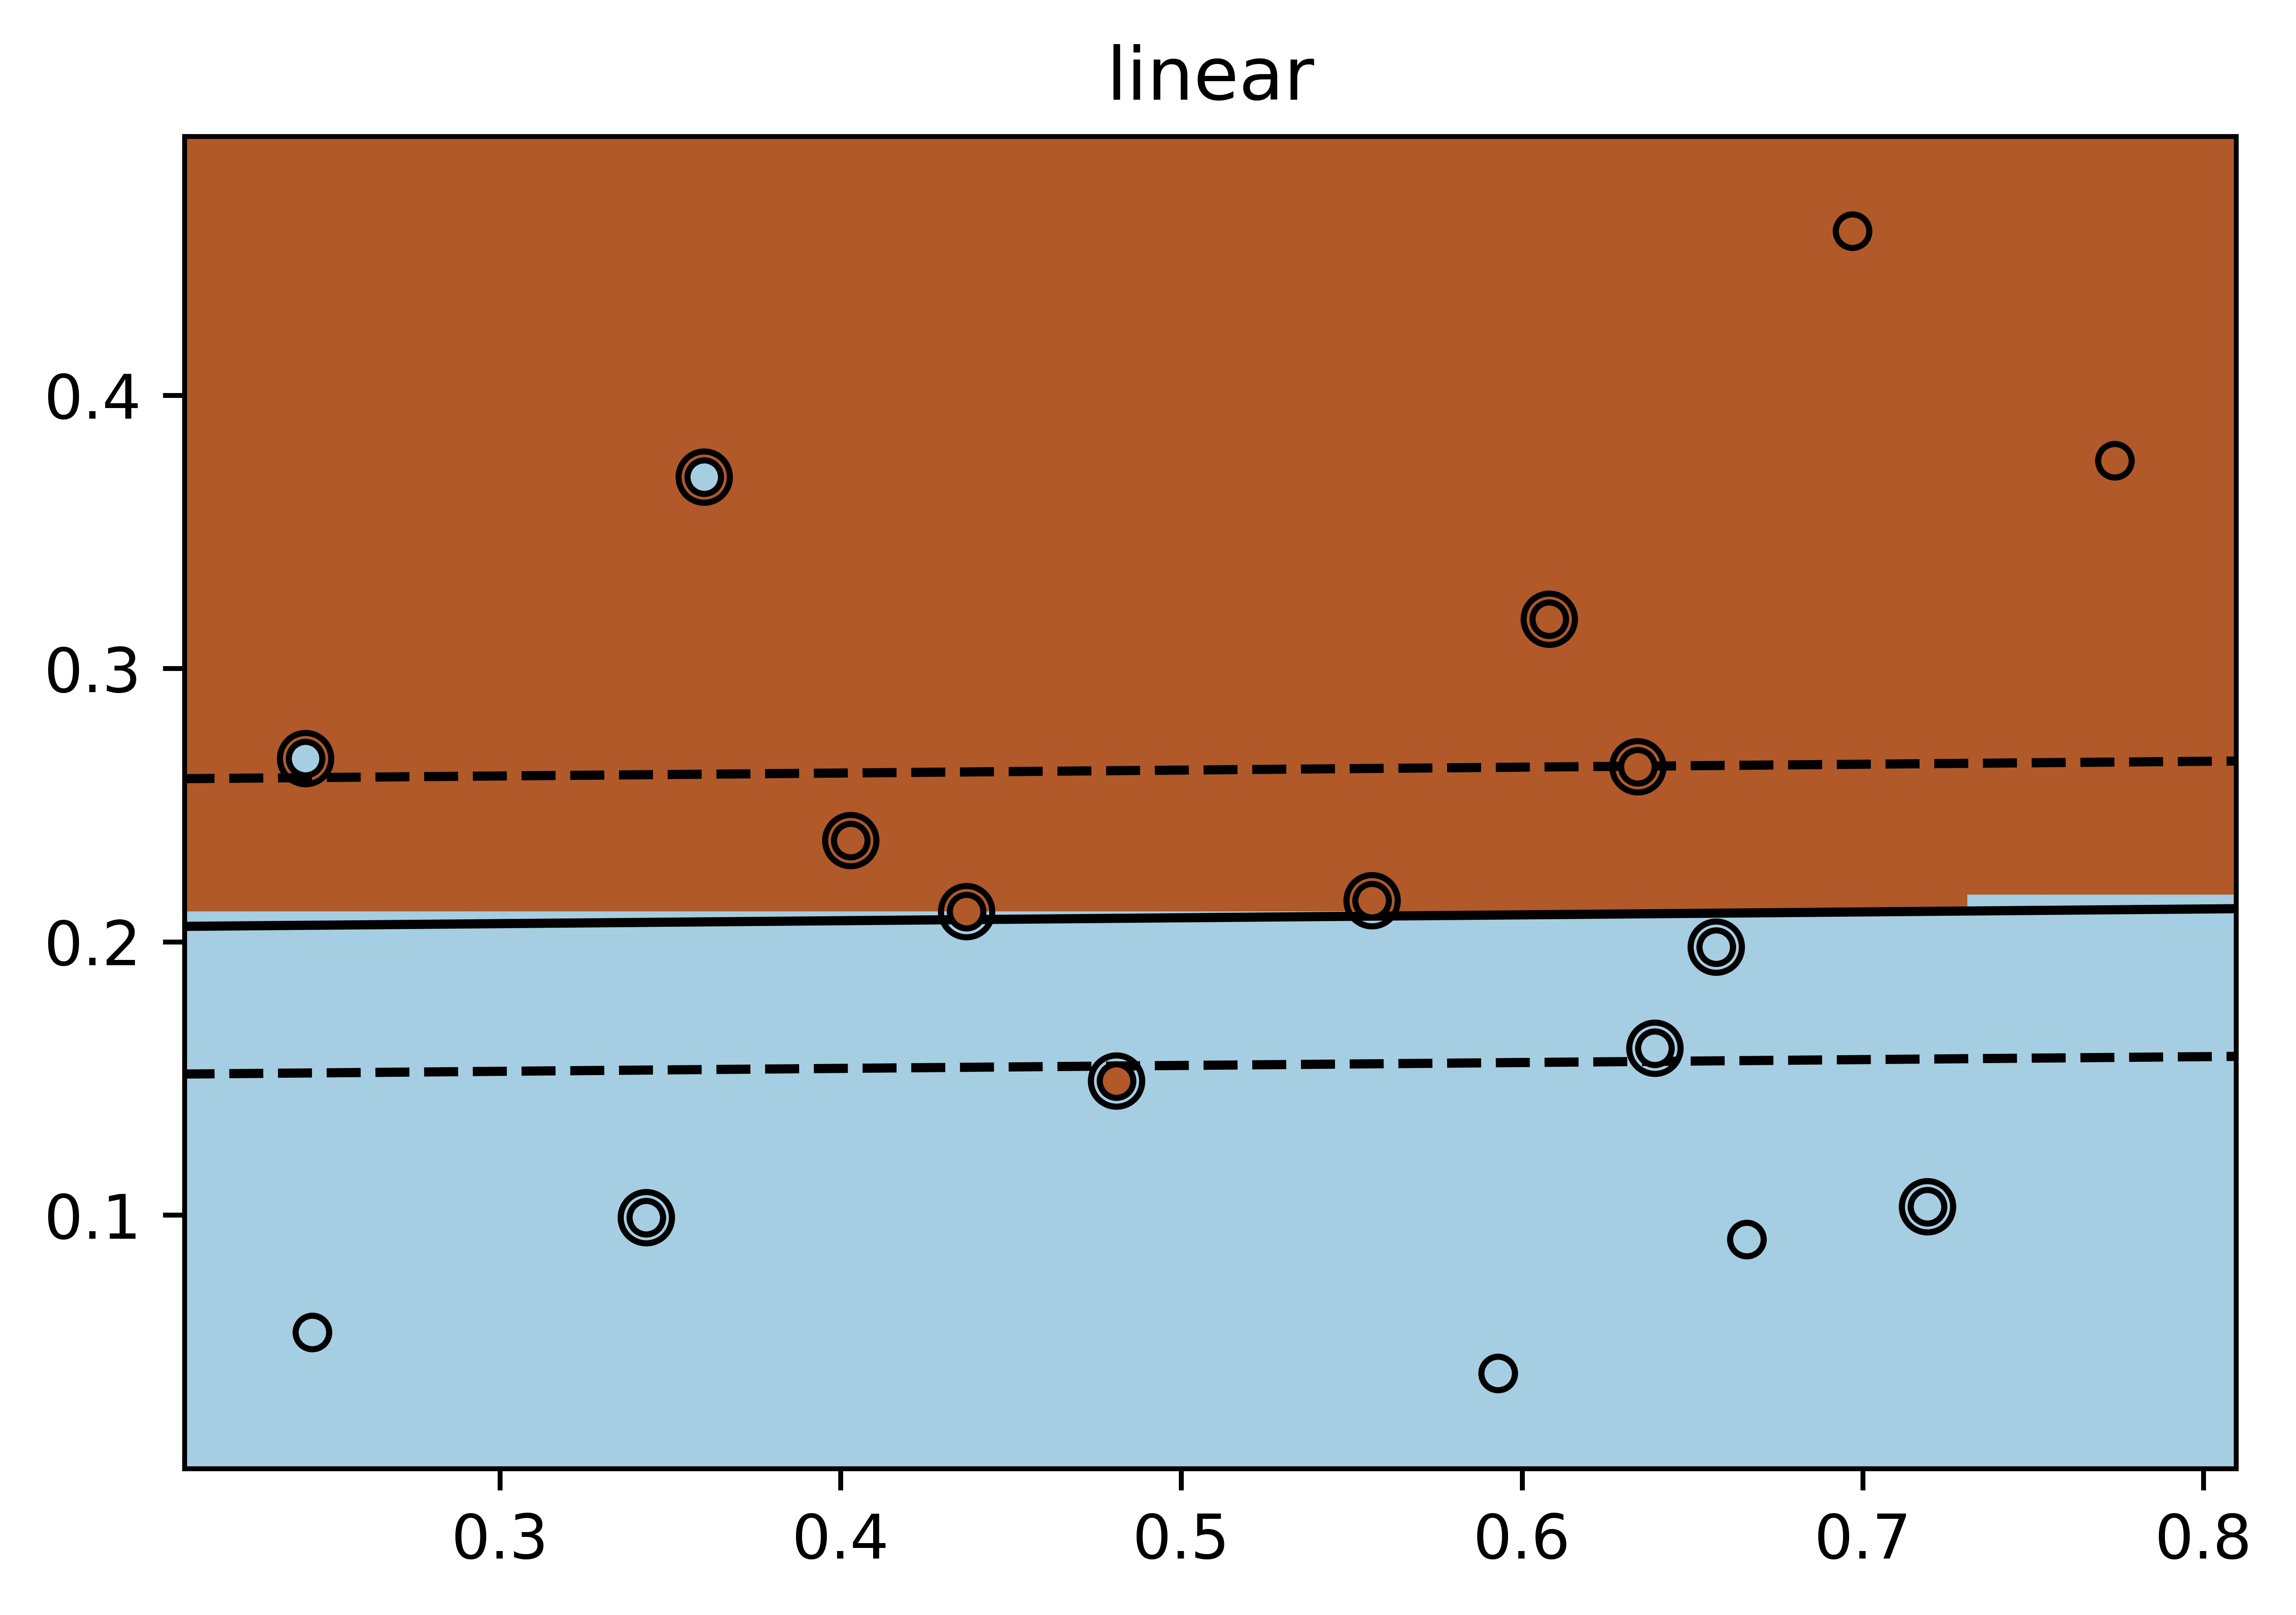
\includegraphics[width=0.7\textwidth]{linear_result.jpg}
	\bicaption{线性核支持向量机训练结果}{Linear kernel SVM training result}
\end{figure}
\par 
根据\textbf{图1},可以看出该线性核支持向量机使用了12个支持向量。在所有样本点中,正确分类且落在间隔边界外8个,正确分类但落在间隔边界内6个,错误分类3个。\par 


使用高斯核训练得到的支持向量机的训练结果如\textbf{图2}所示。

\begin{figure}[h]
	\centering
	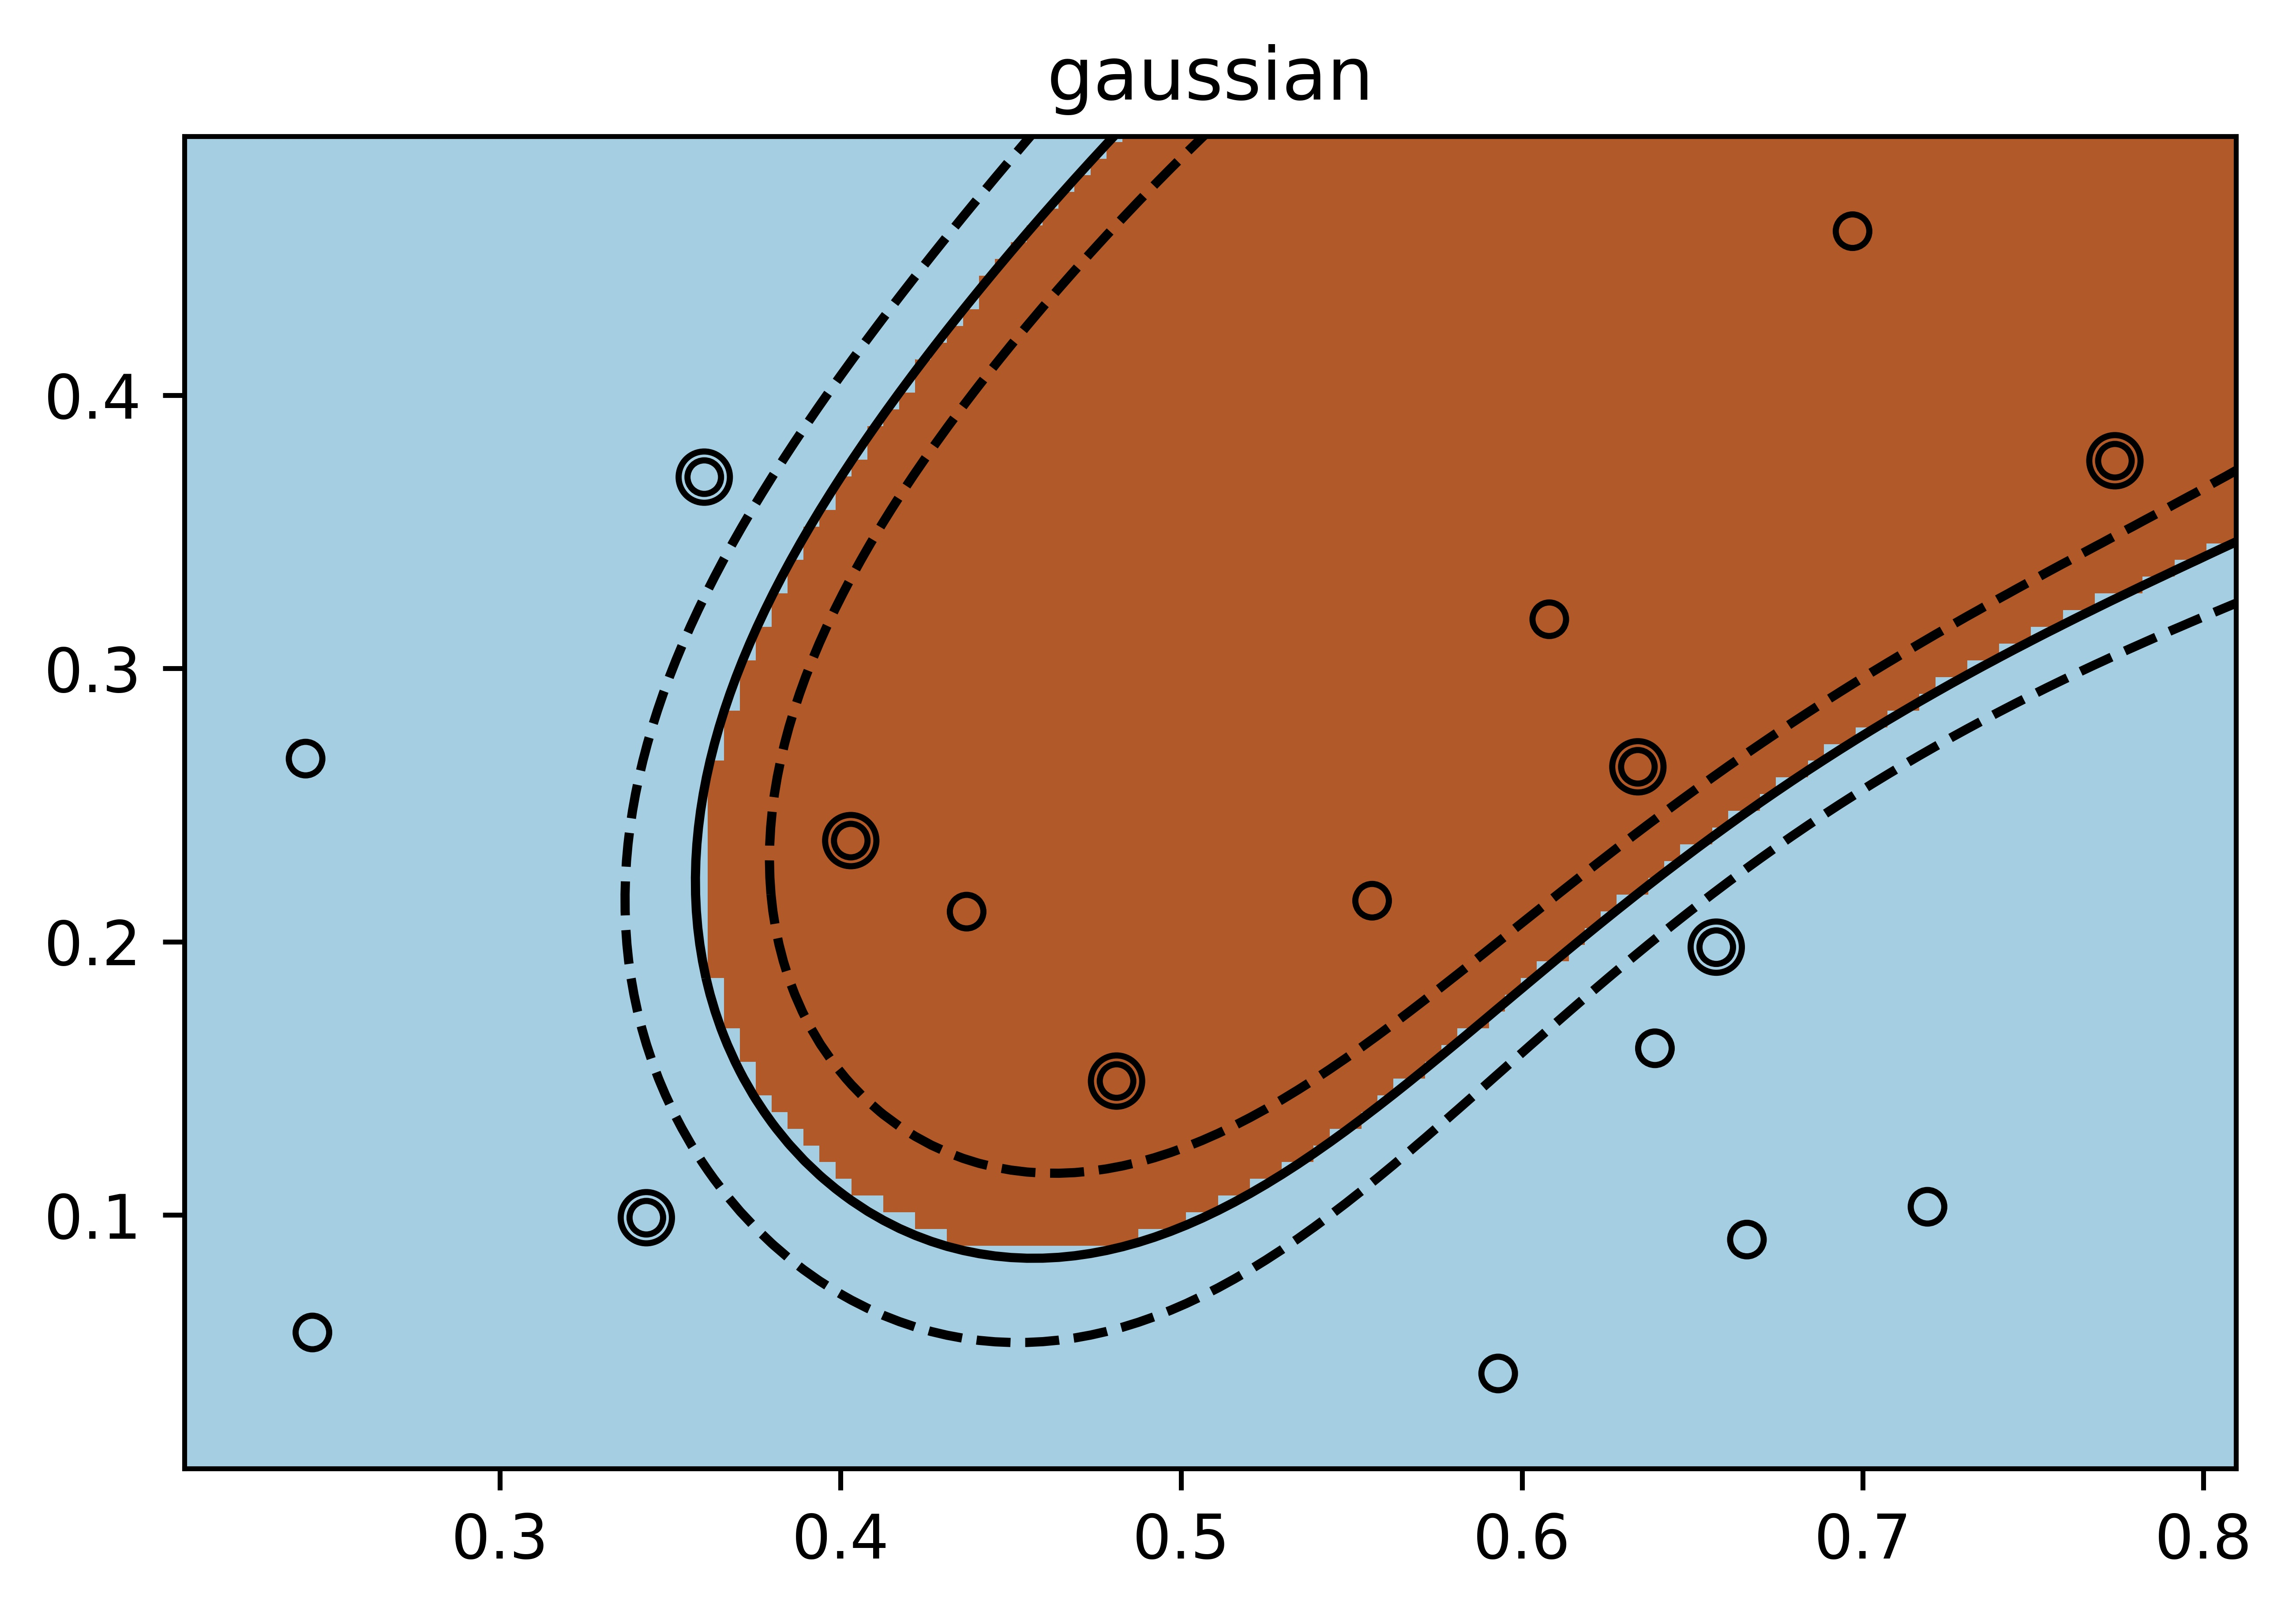
\includegraphics[width=0.7\textwidth]{gaussian_result.jpg}
	\bicaption{高斯核支持向量机训练结果}{Gaussian kernel SVM training result}
\end{figure}
\par 
根据\textbf{图2},可以看出该线性核支持向量机使用了7个支持向量,全部样本点均正确分类且落在间隔边界外。对比\textbf{图1}和\textbf{图2}可以发现,在正则化参数$C$相同时,训练得到的高斯核支持向量机的间隔明显小于线性核支持向量机。
\par

\vbox{}

\subsection{结果分析}
根据1.5的实验结果,可以分析认定:对于本题所用的西瓜数据集$3.0\alpha$,高斯核支持向量机相比线性核支持向量机的间隔更小,因此拟合更好、具有更优的表现;且高斯核支持向量机所用的支持向量数(7个)小于线性核支持向量机(12个),因此具有更快的分类速度和更高的效率。
\vbox{}

\newpage
\section{题目6.10}
\subsection{实验题目}
试设计一个能显著减少SVM中支持向量的数目而不显著降低泛化性能的方法。
\vbox{}
\subsection{实验数据}
题目6.10使用的数据集为scikit-learn库集成的breast\_cancer数据集,该数据集包含了美国Wisconsin州记录的569个乳腺癌病人的恶性/良性数据(以1/0表示),以及与之对应的30维生理指标数据,适用于一般的二分类问题。

\subsection{实验工具}
同1.3,不再赘述。
\vbox{}
\subsection{实验方法}
实验采用1-norm支持向量机算法(1-norm Support Vector Machine)实现显著减少SVM中支持向量的数目而不显著降低泛化性能的要求。1-norm SVM是一种稀疏算法(Sparse Algorithm),能够在不影响模型性能的情况下减少支持向量数目,从而有效提高SVM效率\citealp{jung2013support}。具体地,1-norm SVM具有如下的形式\citealp{zhu20031}:
$$
\min\limits_{\beta_{0}, \beta} \ \ \sum_{i=1}^{n}\Big[1-y_{i}\Big(\beta_{0}+\sum_{j=1}^{q}\beta_{j}h_{j}(x_{i})\Big)\Big]
$$
$$
{\rm s.t.} \ \ ||\beta||_{1}=|\beta_{1}|+\cdots+|\beta_{q}|\leq s
$$
其中$\mathcal{D}={h_{1}(x),\cdots h_{q}(x)}$是一组基函数的集合,$s$是调节参数。得到的模型可以表示为
$$
\hat{f}(x)=\hat{\beta}_{0}+\sum_{j=1}^{q}\hat{\beta}_{j}h_{j}(x)
$$
对应的分类规则由$sign[\hat{f}(x)]$给出。
相比一般的2-norm SVM,1-norm SVM使用L1范数构建惩罚项,能够减少支持向量的数目,有效提高SVM的分类速度。\par 
1-norm SVM的训练可以使用sklearn.LinearSVC库实现,通过指定penalty为l2或l1,可以在一般的2-norm SVM和1-norm SVM间进行切换。实验的具体操作方法如下。首先导入实验所需的必要的库,并读取数据集breast\_cancer的数据;随后定义主体函数LinearSVC\_train,实现对数据集的随机划分、使用划分出的训练集训练SVM、使用测试集对SVM的泛化能力进行检验的功能,并计算SVM所用到的支持向量的个数:
\\
\begin{lstlisting}[language=python]
	from matplotlib import pyplot as plt
	import pandas as pd
	import numpy as np
	
	from sklearn import datasets, svm, metrics
	
	cancer = datasets.load_breast_cancer()
	X = cancer.data
	y = cancer.target
	
	def LinearSVC_train(X, y, penalty='l2', C=1000):
	n_sample = len(X)
	np.random.seed()
	order = np.random.permutation(n_sample)
	X = X[order]
	y = y[order].astype(float)
	
	X_train = X[:int(.9 * n_sample)]
	y_train = y[:int(.9 * n_sample)]
	X_test = X[int(.9 * n_sample):]
	y_test = y[int(.9 * n_sample):]
	
	svc = svm.LinearSVC(C=C, penalty=penalty, dual=False)
	svc.fit(X_train, y_train)
	decision_function = svc.decision_function(X_train)
	support_vector_indices = np.where(np.abs(decision_function) <= 1 + 1e-15)[0]
	support_vector = X_train[support_vector_indices]
	
	y_pred = svc.predict(X_test)
	accuracy = metrics.accuracy_score(y_test, y_pred)
	
	return len(support_vector), accuracy
 \end{lstlisting}
\par 
与1.4类似地,正则化参数$C$通过实验过程中的多次尝试进行选取,$C=1000$基本是较合理的正则化参数。\par 
随后分别训练一般的l2-norm SVM和l1-norm SVM,重复100次,输出两SVM所用到的支持向量个数和预测准确率的平均值:
\begin{lstlisting}[language=python]
	for penalty in ['l2', 'l1']:
		sv_list = []
		accuracy_list = []
	
		for i in range(0, 100):
			sv, ac = LinearSVC_train(X, y, penalty=penalty)
			sv_list.append(sv)
			accuracy_list.append(ac)
	
		print('average number of support vectors ' + '(' + str(penalty) + '-form): ' + str("%.2f" % np.mean(sv_list)))
		print('average accuracy of linear kernel SVM ' + '(' + str(penalty) + '-form): ' + str("%.4f" % np.mean(accuracy_list)))
\end{lstlisting}
\vbox{}
\subsection{实验结果}
实验代码总运行时长为8.96 s。一般的l2-norm SVM和l1-norm SVM的平均支持向量数与平均预测准确率的对比如\textbf{表2}所示。
\begin{table}[h]
	\centering
	\zihao{5}
	\bicaption{l2-norm SVM与l1-norm SVM对比}{Comparison of l2-norm SVM and l1-norm SVM}
	\begin{tabular}{ccc}
		\toprule
		SVM & Average Support Vector Number & Average Accuracy\\
		\midrule
		l2-norm & 83.59 & 0.9588 \\
		l1-norm & 50.35 & 0.9723 \\
		\bottomrule
	\end{tabular}
\end{table}
\par
根据\textbf{表2},可以看出:在breast\_cancer数据集上训练得到的一般的l2-norm SVM所使用的支持向量数的平均值(83.59)明显高于l1-norm SVM(50.35),而在测试集上的平均预测准确率(0.9588)略低于l1-norm SVM(0.9723)。
\subsection{结果分析}
根据2.5的实验结果,可以分析认定:对于本题所用的breast\_cancer数据集,改进后的l1-norm SVM相比一般的l2-norm SVM显著减少了所用支持向量的数目,因此大大提高了分类速度和效率;同时,l1-norm SVM的泛化性能并未降低,在breast\_cancer数据集上的最优表现甚至高于一般的l2-norm SVM。\par 
综合以上结果,可以认为l1-norm SVM算法很好地实现了题目中“显著减少SVM中支持向量数目而不显著降低泛化性能”的要求,具有一定程度的应用价值。

   

\vbox{}

\bibliographystyle{ieeetr}
\bibliography{b}



\end{document}